\documentclass[11pt,a4paper]{article}

% ──────────────────────────────────────────────────────────────────────
% Packages
% ──────────────────────────────────────────────────────────────────────
\usepackage[utf8]{inputenc}
\usepackage[T1]{fontenc}
\usepackage{amsmath,amssymb,amsfonts}
\usepackage{graphicx}
\usepackage{booktabs}
\usepackage{hyperref}
\usepackage{natbib}
\usepackage{listings}
\usepackage{xcolor}
\usepackage{algorithm}
\usepackage{algpseudocode}
\usepackage{multirow}
\usepackage{caption}
\usepackage[margin=1in]{geometry}
\usepackage{tikz}
\usetikzlibrary{arrows.meta,positioning,shapes.geometric,fit,backgrounds}

% ──────────────────────────────────────────────────────────────────────
% Listings style
% ──────────────────────────────────────────────────────────────────────
\definecolor{codebg}{gray}{0.96}
\definecolor{codegreen}{rgb}{0.0,0.5,0.0}
\definecolor{codegray}{rgb}{0.5,0.5,0.5}
\definecolor{codepurple}{rgb}{0.5,0.0,0.5}

\lstdefinestyle{pythonstyle}{
  backgroundcolor=\color{codebg},
  basicstyle=\ttfamily\small,
  breaklines=true,
  commentstyle=\color{codegreen},
  keywordstyle=\color{codepurple}\bfseries,
  stringstyle=\color{codegray},
  numbers=left,
  numberstyle=\tiny\color{codegray},
  numbersep=5pt,
  frame=single,
  language=Python,
  showstringspaces=false,
  captionpos=b,
}
\lstset{style=pythonstyle}

% ──────────────────────────────────────────────────────────────────────
% Title
% ──────────────────────────────────────────────────────────────────────
\title{NeuroSim: A Gymnasium-Compatible Reinforcement Learning\\
       Environment Suite for Brain-Computer Interfaces}

\author{Hass Dhia\\
  Smart Technology Investments Research Institute\\
  Los Angeles, CA, USA\\
  \texttt{partners@smarttechinvest.com}}

\date{\today}

% ══════════════════════════════════════════════════════════════════════
\begin{document}
\maketitle

% ──────────────────────────────────────────────────────────────────────
% 1. ABSTRACT
% ──────────────────────────────────────────────────────────────────────
\begin{abstract}
Brain-computer interface (BCI) research is constrained by the high cost of human
neural recordings, the non-stationarity of neural signals across sessions, and
the absence of standardized reinforcement learning (RL) benchmarks. We present
\textbf{NeuroSim}, an open-source Python library that provides three
Gymnasium-compatible RL environments modeling distinct BCI paradigms:
\texttt{DecoderAdapt-v0} for motor imagery decoder adaptation,
\texttt{CursorControl-v0} for continuous intracortical cursor control, and
\texttt{SpellerNav-v0} for P300-based speller stimulus selection. Each
environment incorporates physiologically grounded signal models for electrode
impedance drift, neural fatigue, feature distribution shifts, and
user--decoder co-adaptation. NeuroSim integrates with the MOABB dataset
ecosystem for calibration from real EEG data and includes a conditional
variational autoencoder (cVAE) surrogate for generating unlimited synthetic
training epochs. We report baseline results with Proximal Policy Optimization
(PPO) trained for 20,000 timesteps across all three environments. PPO
achieves a mean reward of 121.11 on DecoderAdapt-v0 (vs.\ 23.70 for a random
agent) and $-89.99$ on CursorControl-v0 (vs.\ $-209.21$), while
underperforming random on SpellerNav-v0 ($-11.60$ vs.\ $-5.55$) due to
insufficient exploration at this training budget. The platform also provides a
classical CSP+LDA baseline for comparison with RL agents and a leave-one-subject-out
cross-subject transfer evaluation protocol. The full platform, including
158 passing tests and benchmark infrastructure, is released under the MIT
license at \url{https://github.com/HassDhia/neurosim}.
\end{abstract}

% ──────────────────────────────────────────────────────────────────────
% 2. INTRODUCTION
% ──────────────────────────────────────────────────────────────────────
\section{Introduction}
\label{sec:introduction}

Brain-computer interfaces translate neural activity into control signals for
external devices, enabling communication and motor restoration for individuals
with severe neurological conditions. Despite substantial progress in neural
decoding algorithms, BCI systems remain fragile in practice: electrode
impedance drifts over hours, neural signal statistics shift across sessions,
and users co-adapt their neural strategies to the decoder's expectations.
These non-stationarities degrade decoder performance and necessitate frequent
recalibration, reducing the usability of BCI systems in real-world settings.

Reinforcement learning offers a principled framework for addressing these
challenges. An RL agent can learn adaptive policies that respond to signal
degradation, balance exploration against exploitation in stimulus selection,
and manage the cost--benefit tradeoff of decoder recalibration. However,
training RL agents on real neural data is prohibitively expensive and
ethically constrained. Each experimental session requires a human participant,
specialized recording equipment, and hours of setup time. Simulated
environments offer an alternative, but existing BCI simulation tools lack the
standardized interfaces, signal fidelity, and benchmark infrastructure needed
for rigorous RL research.

This paper introduces \textbf{NeuroSim}, a Gymnasium-compatible environment
suite designed to bridge this gap. NeuroSim makes three contributions:

\begin{enumerate}
  \item \textbf{Three standardized RL environments} covering the primary BCI
    paradigms---motor imagery classification, continuous cursor control, and
    event-related potential (ERP) speller navigation---each with carefully
    designed observation, action, and reward spaces.
  \item \textbf{Physiologically grounded signal models} for four sources of
    non-stationarity (electrode impedance drift, neural fatigue, feature
    distribution shift, and user--decoder co-adaptation), composable through a
    modular signal pipeline.
  \item \textbf{A conditional VAE surrogate} trained on real or synthetic
    neural epochs that provides unlimited class-conditioned data generation
    for scalable RL training.
  \item \textbf{Classical and cross-subject baselines}: a CSP+LDA
    classifier for comparison with RL agents, and a leave-one-subject-out
    (LOSO) transfer evaluation protocol for assessing generalization
    across synthetic subject cohorts.
\end{enumerate}

NeuroSim integrates with the MOABB dataset ecosystem \citep{jayaram2018moabb}
for calibration from real recordings and provides a benchmark runner with
PPO baselines for reproducible comparisons. The entire platform is released
as an installable Python package under the MIT license with 158 passing tests,
type annotations, and comprehensive documentation.

The remainder of this paper is organized as follows. Section~\ref{sec:related}
reviews related work in BCI simulation and RL for neural decoding.
Section~\ref{sec:architecture} describes the system architecture.
Section~\ref{sec:environments} details the three Gymnasium environments.
Section~\ref{sec:signal-models} formalizes the signal models.
Section~\ref{sec:surrogate} presents the cVAE surrogate architecture.
Section~\ref{sec:experiments} reports baseline PPO results.
Section~\ref{sec:discussion} discusses design tradeoffs and limitations.
Section~\ref{sec:conclusion} concludes with a summary and future directions.

% ──────────────────────────────────────────────────────────────────────
% 3. RELATED WORK
% ──────────────────────────────────────────────────────────────────────
\section{Related Work}
\label{sec:related}

\subsection{BCI Simulators}

Simulation has long been recognized as essential for BCI algorithm
development, but few platforms provide the combination of physiological
fidelity and RL-ready interfaces. \citet{liang2024bci} provided a
comprehensive review of BCI simulator architectures, identifying key gaps in
signal non-stationarity modeling and standardized benchmarking. Their work
highlighted the need for modular simulation components that can be composed
to model different BCI paradigms and degradation scenarios.

Existing tools for BCI data access include MOABB \citep{jayaram2018moabb},
which standardizes access to 36+ BCI datasets through a unified Python API
covering motor imagery, P300, and steady-state visual evoked potential
(SSVEP) paradigms. BrainFlow provides a hardware abstraction layer for
real-time neural data acquisition but does not include simulation capabilities.
NeuroGym offers Gymnasium-compatible neuroscience environments, but focuses on
cognitive neuroscience tasks rather than BCI-specific signal processing
challenges.

NeuroSim differentiates itself by combining MOABB's dataset ecosystem with
physiologically grounded non-stationarity models and RL-native environment
interfaces. Rather than replacing existing tools, NeuroSim builds on them:
MOABB data feeds the signal models, which in turn drive the Gymnasium
environments.

\subsection{Reinforcement Learning for BCI}

The application of RL to BCI control has been explored from multiple angles.
\citet{kao2025copilots} demonstrated that RL agents can learn to co-adapt with
neural decoders, improving closed-loop performance beyond what fixed decoding
algorithms achieve. Their work established the theoretical framework for
treating BCI control as a partially observable Markov decision process.

\citet{sanchez2009rlbmi} initiated the study of reinforcement learning
architectures for brain-machine interfaces, showing that RL agents can learn
co-adaptive decoder strategies from reward signals alone. Their work on
exploiting co-adaptation for symbiotic neuroprosthetic assistants demonstrated
that the user and decoder can be modeled as a coupled dynamical system where
both parties adapt simultaneously.

The Co-adaptive Policy Actor-Critic (CopAC) framework \citep{copac2024}
formalized the co-adaptation problem as a two-player cooperative game between
the user and the decoder, each modeled as an RL agent. This perspective
directly informs NeuroSim's co-adaptation model, which simulates the user's
side of this interaction.

Despite these advances, RL for BCI research has been hampered by the lack of
standardized benchmarks. Each study uses different datasets, signal processing
pipelines, and evaluation metrics, making cross-study comparisons difficult.
NeuroSim addresses this gap by providing a common evaluation framework with
fixed environment specifications and baseline agent comparisons.

\subsection{Gymnasium Ecosystem}

The Gymnasium API \citep{brockman2016gym} (originally OpenAI Gym) has become
the de facto standard for RL environment interfaces. Its \texttt{reset()}/\texttt{step()}
protocol, coupled with standardized observation and action spaces, enables
algorithm-agnostic benchmarking. NeuroSim adopts this interface wholesale,
ensuring compatibility with popular RL libraries such as Stable Baselines3
\citep{raffin2021sb3}, RLlib, and CleanRL. Each NeuroSim environment registers
under the \texttt{neurosim/} namespace and can be instantiated via
\texttt{gymnasium.make()}.

% ──────────────────────────────────────────────────────────────────────
% 4. SYSTEM ARCHITECTURE
% ──────────────────────────────────────────────────────────────────────
\section{System Architecture}
\label{sec:architecture}

NeuroSim is organized as a layered Python package with clear separation between
data ingestion, signal modeling, environment simulation, and agent training.
Figure~\ref{fig:architecture} illustrates the data flow through the system.

\begin{figure}[ht]
  \centering
  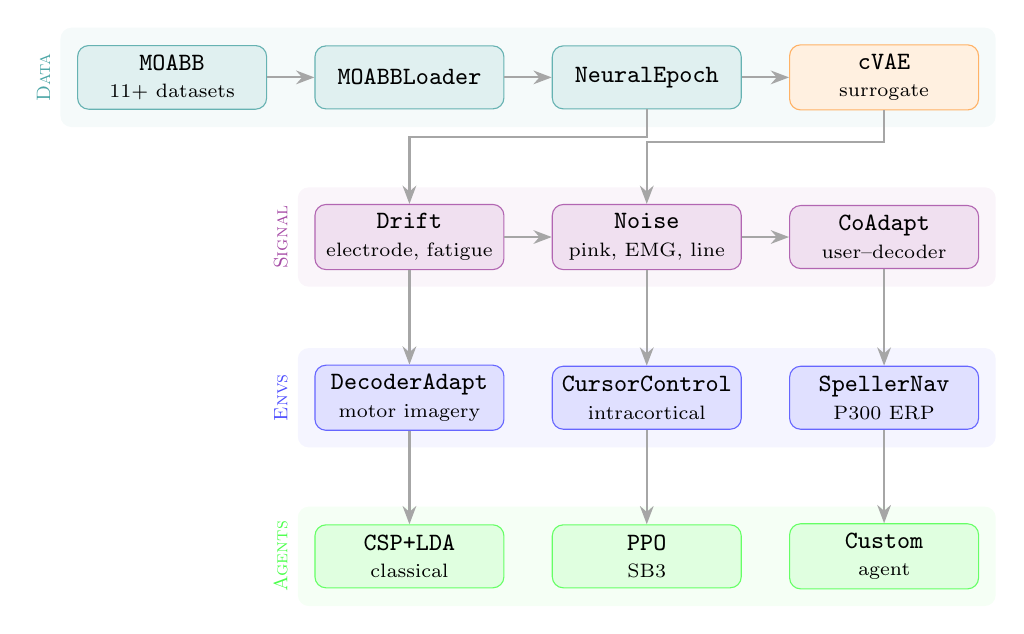
\begin{tikzpicture}[
    >=Stealth,
    node distance=0.9cm and 0.6cm,
    every node/.style={font=\small},
    block/.style={draw, rounded corners, minimum height=0.8cm, minimum width=2.4cm,
                  fill=#1!12, draw=#1!60, align=center},
    block/.default=blue,
    lbl/.style={font=\scriptsize\sffamily, text=#1!70},
    lbl/.default=black,
    arr/.style={->, thick, draw=gray!70},
  ]
    % --- Data layer ---
    \node[block=teal]                     (moabb)  {\texttt{MOABB}\\[-1pt]\scriptsize 11+ datasets};
    \node[block=teal, right=of moabb]     (loader) {\texttt{MOABBLoader}};
    \node[block=teal, right=of loader]    (epoch)  {\texttt{NeuralEpoch}};
    \node[block=orange, right=of epoch]   (cvae)   {\texttt{cVAE}\\[-1pt]\scriptsize surrogate};

    % --- Signal layer ---
    \node[block=violet, below=1.2cm of loader] (drift)  {\texttt{Drift}\\[-1pt]\scriptsize electrode, fatigue};
    \node[block=violet, right=of drift]        (noise)  {\texttt{Noise}\\[-1pt]\scriptsize pink, EMG, line};
    \node[block=violet, right=of noise]        (coadapt){\texttt{CoAdapt}\\[-1pt]\scriptsize user--decoder};

    % --- Environment layer ---
    \node[block=blue, below=1.2cm of drift]    (decode) {\texttt{DecoderAdapt}\\[-1pt]\scriptsize motor imagery};
    \node[block=blue, right=of decode]         (cursor) {\texttt{CursorControl}\\[-1pt]\scriptsize intracortical};
    \node[block=blue, right=of cursor]         (spell)  {\texttt{SpellerNav}\\[-1pt]\scriptsize P300 ERP};

    % --- Agent layer ---
    \node[block=green, below=1.2cm of cursor]  (ppo)    {\texttt{PPO}\\[-1pt]\scriptsize SB3};
    \node[block=green, left=of ppo]            (csp)    {\texttt{CSP+LDA}\\[-1pt]\scriptsize classical};
    \node[block=green, right=of ppo]           (custom) {\texttt{Custom}\\[-1pt]\scriptsize agent};

    % --- Arrows: data flow ---
    \draw[arr] (moabb)  -- (loader);
    \draw[arr] (loader) -- (epoch);
    \draw[arr] (epoch)  -- (cvae);
    \draw[arr] (cvae.south) -- ++(0,-0.4) -| (noise.north);
    \draw[arr] (epoch.south) -- ++(0,-0.35) -| (drift.north);

    % --- Signal pipeline arrows ---
    \draw[arr] (drift) -- (noise);
    \draw[arr] (noise) -- (coadapt);

    % --- Signal to envs ---
    \draw[arr] (drift.south)   -- (decode.north);
    \draw[arr] (noise.south)   -- (cursor.north);
    \draw[arr] (coadapt.south) -- (spell.north);

    % --- Envs to agents ---
    \draw[arr] (decode.south) -- (csp.north);
    \draw[arr] (cursor.south) -- (ppo.north);
    \draw[arr] (spell.south)  -- (custom.north);

    % --- Layer labels ---
    \begin{scope}[on background layer]
      \node[fit=(moabb)(cvae), inner sep=6pt, fill=teal!4, rounded corners,
            label={[lbl=teal]left:\rotatebox{90}{\textsc{Data}}}] {};
      \node[fit=(drift)(coadapt), inner sep=6pt, fill=violet!4, rounded corners,
            label={[lbl=violet]left:\rotatebox{90}{\textsc{Signal}}}] {};
      \node[fit=(decode)(spell), inner sep=6pt, fill=blue!4, rounded corners,
            label={[lbl=blue]left:\rotatebox{90}{\textsc{Envs}}}] {};
      \node[fit=(csp)(custom), inner sep=6pt, fill=green!4, rounded corners,
            label={[lbl=green]left:\rotatebox{90}{\textsc{Agents}}}] {};
    \end{scope}
  \end{tikzpicture}
  \caption{NeuroSim system architecture. Data flows top-to-bottom through four
    layers: real EEG from MOABB is converted to \texttt{NeuralEpoch} objects
    (with optional cVAE augmentation), processed through a composable signal
    pipeline of drift, noise, and co-adaptation models, served to three
    Gymnasium environments, and acted upon by RL or classical agents via the
    standard \texttt{step()} interface.}
  \label{fig:architecture}
\end{figure}

\subsection{Data Pipeline}

The data pipeline bridges the MOABB ecosystem into NeuroSim's internal
representation. The \texttt{MOABBLoader} class wraps MOABB's dataset and
paradigm API, converting raw EEG recordings into a flat list of
\texttt{NeuralEpoch} objects---a standardized dataclass containing signal
arrays of shape $(C \times T)$ (channels by timepoints), integer class
labels, sampling frequency, channel names, and subject/session identifiers.

MOABB and MNE are specified as optional dependencies
(\texttt{pip install neurosim[data]}), so the core simulation functionality
operates without them. When MOABB is unavailable, environments generate
synthetic neural signals using built-in noise models. The loader supports
eight priority datasets spanning the major BCI paradigms:

\begin{itemize}
  \item BNCI2014\_001: 9 subjects, 2 sessions, 4-class motor imagery
  \item BNCI2014\_004: 9 subjects, 5 sessions, 2-class motor imagery
  \item BNCI2015\_001: 12 subjects, 2--3 sessions, 2-class motor imagery
  \item Cho2017: 52 subjects, 1 session, 2-class motor imagery
  \item Lee2019\_MI: 54 subjects, 2 sessions, 2-class motor imagery
  \item PhysionetMI: 109 subjects, 1 session, 4-class motor imagery
  \item Weibo2014: 10 subjects, 1 session, 7-class motor imagery
  \item Zhou2016: 4 subjects, 3 sessions, 3-class motor imagery
\end{itemize}

A preprocessing module provides standard EEG preprocessing operations---bandpass
filtering, common average referencing (CAR), z-score normalization, and artifact
rejection---composable into a \texttt{preprocess\_pipeline} function.

Feature extraction converts \texttt{NeuralEpoch} objects into environment
observation vectors. The \texttt{extract\_band\_power} function computes power
spectral density via Welch's method across five standard EEG frequency bands
(delta: 0.5--4~Hz, theta: 4--8~Hz, alpha: 8--13~Hz, beta: 13--30~Hz,
gamma: 30--45~Hz). The \texttt{extract\_log\_variance} function computes
per-channel log-variance, a robust feature inspired by Common Spatial Patterns
(CSP).

\subsection{Environment Design Philosophy}

NeuroSim environments follow three design principles:

\textbf{Plug-in signal models.} Each environment accepts an optional
\texttt{signal\_pipeline} parameter of type \texttt{SignalPipeline}. When
\texttt{None} (the default), the environment uses built-in inline noise
generation. This ensures that the default behavior is unchanged when no
pipeline is provided, while allowing researchers to inject arbitrary
combinations of drift, noise, and co-adaptation models.

\textbf{Dict observation and action spaces.} Environments use Gymnasium's
\texttt{Dict} spaces to expose semantically meaningful observation components
(e.g., \texttt{neural\_features}, \texttt{decoder\_confidence},
\texttt{cursor\_position}) and structured actions (e.g., simultaneous
classification and recalibration decisions). For compatibility with RL
libraries that require flat spaces, NeuroSim provides a
\texttt{FlattenDictActionWrapper} and an \texttt{ObservationFlattener} utility.

\textbf{Gymnasium registration.} All environments register under the
\texttt{neurosim/} namespace and can be instantiated via
\texttt{gymnasium.make("neurosim/DecoderAdapt-v0")}. This enables seamless
integration with standard RL training loops.

\subsection{Dependency Architecture}

NeuroSim uses a tiered dependency structure to minimize installation burden:

\begin{itemize}
  \item \textbf{Core} (\texttt{pip install neurosim}): NumPy $\geq$1.24,
    SciPy $\geq$1.11, Gymnasium $\geq$0.29. All environments and signal
    models are fully functional with only these dependencies.
  \item \textbf{Data} (\texttt{neurosim[data]}): MNE $\geq$1.6, MOABB
    $\geq$1.0. Required only for loading real EEG datasets.
  \item \textbf{Surrogate} (\texttt{neurosim[surrogate]}): PyTorch $\geq$2.0.
    Required only for the cVAE surrogate model.
  \item \textbf{Training} (\texttt{neurosim[train]}): Stable Baselines3
    $\geq$2.0, PyTorch $\geq$2.0. Required only for the PPO training script.
\end{itemize}

This design ensures that importing \texttt{neurosim.envs} never triggers
PyTorch or MOABB imports, keeping the core package lightweight. PyTorch is
imported lazily inside the \texttt{NeuralSurrogate} class only when
\texttt{train()} or \texttt{load()} is called.

% ──────────────────────────────────────────────────────────────────────
% 5. GYMNASIUM ENVIRONMENTS
% ──────────────────────────────────────────────────────────────────────
\section{Gymnasium Environments}
\label{sec:environments}

NeuroSim provides three environments that model distinct BCI paradigms. Each
environment defines observation spaces, action spaces, reward functions, and
episode structures that capture the essential challenges of its paradigm.

% ──────────────────────────────────────
\subsection{DecoderAdapt-v0}
\label{sec:decoder-adapt}

The \texttt{DecoderAdapt-v0} environment models the motor imagery BCI decoder
adaptation problem. The agent receives neural features and must simultaneously
classify the imagined movement, decide whether to trigger a costly
recalibration, and set the online adaptation rate. This captures the real-world
tradeoff where decoder drift degrades accuracy over time, but recalibration
interrupts the user's workflow.

\textbf{Observation space.}
The observation is a dictionary with six components:

\begin{itemize}
  \item \texttt{neural\_features} $(24,)$: Band-power and CSP-derived features
    from EEG, reflecting the current class-conditioned neural activity plus
    drift and noise.
  \item \texttt{decoder\_confidence} $(4,)$: Softmax output of the simulated
    decoder, providing a probability distribution over the four motor imagery
    classes.
  \item \texttt{decoder\_age} $(1,)$: Normalized count of steps since the last
    recalibration, indicating how stale the current decoder parameters are.
  \item \texttt{session\_progress} $(1,)$: Fraction of the episode elapsed,
    enabling time-aware policies.
  \item \texttt{recent\_accuracy} $(1,)$: Rolling classification accuracy over
    the last 20 trials.
  \item \texttt{drift\_indicator} $(24,)$: Absolute difference between the
    current feature distribution mean and the calibration distribution mean,
    serving as an explicit signal of distribution shift.
\end{itemize}

The total observation dimensionality is 55 when flattened.

\textbf{Action space.}
The action is a dictionary with three components:

\begin{itemize}
  \item \texttt{classification}: $\mathrm{Discrete}(4)$ --- the predicted
    motor imagery class.
  \item \texttt{recalibrate}: $\mathrm{Discrete}(2)$ --- 0 to keep the current
    decoder, 1 to trigger recalibration.
  \item \texttt{adaptation\_rate}: $\mathrm{Box}(1) \in [0, 1]$ --- continuous
    online learning rate controlling how aggressively the decoder adapts to
    recent data.
\end{itemize}

For compatibility with Stable Baselines3, the \texttt{FlattenDictActionWrapper}
converts this into a $\mathrm{Box}(6)$ space where discrete actions are encoded
as continuous values and rounded back to integers during execution.

\textbf{Reward function.}
\begin{equation}
  r_t = \underbrace{+1.0}_{\text{correct}} +
        \underbrace{+0.2 \cdot \mathbb{1}[\text{streak} \geq 5]}_{\text{streak bonus}} -
        \underbrace{0.3 \cdot \mathbb{1}[\text{recalibrate}]}_{\text{recalibration cost}}
  \label{eq:decoder-reward}
\end{equation}

The agent receives $+1.0$ for each correct classification, a $+0.2$ streak
bonus when five or more consecutive classifications are correct, and incurs a
$-0.3$ penalty each time it triggers recalibration.

\textbf{Episode structure.}
Each episode consists of 300 steps (trials). At each step, a motor imagery
class is sampled uniformly from the four classes. The environment simulates
feature distribution drift at a configurable rate, shifting the calibration
mean away from the current distribution. The episode terminates by truncation
after 300 steps.

% ──────────────────────────────────────
\subsection{CursorControl-v0}
\label{sec:cursor-control}

The \texttt{CursorControl-v0} environment models intracortical BCI cursor
control, inspired by BrainGate-style systems where a population of motor
cortex neurons encodes intended movement direction and speed. The agent decodes
neural population activity into 2D velocity commands to acquire screen
targets.

\textbf{Observation space.}
The observation is a dictionary with six components:

\begin{itemize}
  \item \texttt{neural\_state} $(96, 5)$: Simulated spike counts from 96
    neural units across 5 time bins. Neural activity follows a cosine tuning
    model where each unit's firing rate depends on the cosine similarity
    between the intended movement direction and the unit's preferred direction.
  \item \texttt{cursor\_position} $(2,)$: Current cursor $[x, y]$ in a
    normalized $[0, 1] \times [0, 1]$ workspace.
  \item \texttt{target\_position} $(2,)$: Target $[x, y]$ coordinates.
  \item \texttt{cursor\_velocity} $(2,)$: Current velocity vector.
  \item \texttt{distance\_to\_target} $(1,)$: Euclidean distance to the
    target.
  \item \texttt{time\_in\_trial} $(1,)$: Fraction of maximum trial steps
    elapsed.
\end{itemize}

\textbf{Action space.}
$\mathrm{Box}(2) \in [-1, 1]$: a two-dimensional decoded velocity command
$[v_x, v_y]$ that displaces the cursor by $\mathbf{v} \cdot 0.05$ per step,
clamped to the workspace boundaries.

\textbf{Reward function.}
\begin{equation}
  r_t = \underbrace{-0.01 \cdot d_t}_{\text{distance}} +
        \underbrace{1.0 \cdot \Delta d_t}_{\text{progress}} +
        \underbrace{5.0 \cdot \mathbb{1}[\text{acquire}]}_{\text{acquisition}} -
        \underbrace{0.1 \cdot \|\mathbf{v}_t - \mathbf{v}_{t-1}\|}_{\text{jitter}}
  \label{eq:cursor-reward}
\end{equation}

where $d_t$ is the Euclidean distance to the target, $\Delta d_t = d_{t-1} -
d_t$ is the progress toward the target, and the jitter penalty discourages
erratic velocity changes. The acquisition bonus is scaled by time efficiency:
$5.0 \cdot (1 - 0.5 \cdot t_\text{trial}/t_\text{max})$, rewarding faster
reaches.

\textbf{Episode structure.}
Each episode consists of 50 reach trials. Within each trial, the agent has up
to 30 steps to move the cursor within a radius of 0.05 of the target. A trial
ends upon target acquisition or timeout, after which a new target is sampled.
The cursor resets to the workspace center $(0.5, 0.5)$ at the start of each
trial, and targets are sampled uniformly from $[0.1, 0.9]^2$ with a minimum
distance of 0.2 from the cursor.

% ──────────────────────────────────────
\subsection{SpellerNav-v0}
\label{sec:speller-nav}

The \texttt{SpellerNav-v0} environment models an active-query BCI speller
where the agent controls which stimulus groups to flash and decides when to
commit to a symbol selection. This captures the explore--exploit tradeoff in
ERP-based BCIs: more flashes improve classification accuracy but reduce the
information transfer rate (ITR).

\textbf{Observation space.}
The observation is a dictionary with five components:

\begin{itemize}
  \item \texttt{posterior} $(36,)$: Bayesian posterior probability distribution
    over the 36-symbol alphabet (A--Z, 0--9).
  \item \texttt{response\_history} $(10, 8)$: The last 10 ERP responses across
    8 EEG channels, providing temporal context for evidence accumulation.
  \item \texttt{n\_flashes} $(1,)$: Number of flashes used for the current
    symbol, normalized by the maximum (30).
  \item \texttt{target\_queue} $(5,)$: Indices of the upcoming target symbols
    in the word to be spelled.
  \item \texttt{snr\_estimate} $(1,)$: Estimated signal-to-noise ratio
    computed from the response buffer.
\end{itemize}

\textbf{Action space.}
The action is a dictionary with two components:

\begin{itemize}
  \item \texttt{stimulus\_group}: $\mathrm{Discrete}(6)$ --- selects which of
    the 6 groups (each containing $36/6 = 6$ symbols) to flash.
  \item \texttt{commit}: $\mathrm{Discrete}(2)$ --- 0 to continue flashing,
    1 to commit to the maximum a posteriori (MAP) symbol.
\end{itemize}

For SB3 compatibility, the \texttt{FlattenDictActionWrapper} converts this to
$\mathrm{MultiDiscrete}([6, 2])$.

\textbf{Reward function.}
\begin{equation}
  r_t = \underbrace{-0.02}_{\text{per flash}} +
        \underbrace{+3.0 \cdot \mathbb{1}[\text{correct commit}]}_{\text{correct}} +
        \underbrace{(-2.0) \cdot \mathbb{1}[\text{wrong commit}]}_{\text{wrong}}
  \label{eq:speller-reward}
\end{equation}

Each flash incurs a small cost of $-0.02$, incentivizing efficient evidence
accumulation. A correct commit earns $+3.0$ and an incorrect commit incurs
$-2.0$. An additional ITR bonus proportional to $(1 - n_\text{flashes}/30)$
rewards faster decisions when correct. If the agent exhausts the maximum of
30 flashes without committing, a forced commit occurs with a reduced
correct bonus of $+1.5$.

\textbf{Episode structure.}
Each episode requires spelling 5 symbols. For each symbol, the agent may
flash up to 30 times before a forced commit. The simulated ERP response uses a
spatial P300 pattern: when the target symbol is in the flashed group, a
positive deflection with spatial gradient $[0.3, 0.5, 0.8, 1.0, 1.0, 0.8,
0.5, 0.3]$ across channels is added, scaled by a configurable amplitude
(default 1.5). The posterior is updated via Bayesian inference after each flash.

\subsection{Environment Summary}

Table~\ref{tab:env-summary} summarizes the key specifications of all three
environments.

\begin{table}[ht]
  \centering
  \caption{Summary of NeuroSim environment specifications.}
  \label{tab:env-summary}
  \begin{tabular}{@{}lccc@{}}
    \toprule
    \textbf{Property} & \textbf{DecoderAdapt-v0} & \textbf{CursorControl-v0} & \textbf{SpellerNav-v0} \\
    \midrule
    BCI Paradigm & Motor imagery & Intracortical & P300 speller \\
    Obs.\ Dim.\ (flat) & 55 & 488 & 128 \\
    Action Type & Dict (mixed) & Box(2) & Dict (discrete) \\
    Episode Length & 300 steps & 50 trials $\times$ 30 & 5 symbols $\times$ 30 \\
    Signal Model & Feature drift & Cosine tuning & P300 + Bayesian \\
    \bottomrule
  \end{tabular}
\end{table}

% ──────────────────────────────────────────────────────────────────────
% 6. SIGNAL MODELS
% ──────────────────────────────────────────────────────────────────────
\section{Signal Models}
\label{sec:signal-models}

Real BCI signals are affected by multiple sources of non-stationarity that
degrade decoder performance over time. NeuroSim models four such sources,
each implemented as an independent module that can be composed through the
\texttt{SignalPipeline} class. The pipeline applies models in a
physiologically motivated order: drift models first (electrode and neural
degradation), then noise injection (environmental and physiological
artifacts), and finally co-adaptation (user learning).

\subsection{Electrode Impedance Drift}

Electrode impedance increases over time due to gel drying, electrode
displacement, and skin conductance changes. Higher impedance attenuates the
recorded signal amplitude. The \texttt{ElectrodeDriftModel} simulates this
process:

\begin{equation}
  Z(t) = Z_0 \cdot \left(1 + \alpha_z \cdot t + \epsilon_z(t)\right)
  \label{eq:impedance}
\end{equation}
\begin{equation}
  \text{signal}_\text{out} = \text{signal}_\text{in} \cdot \frac{Z_0}{Z(t)}
  \label{eq:impedance-attenuation}
\end{equation}

where $\alpha_z$ is the linear drift rate per timestep (default 0.001),
$\epsilon_z(t) \sim \mathcal{N}(0, \sigma_z^2)$ is per-channel impedance
noise with $\sigma_z = 0.01$, and $Z_0$ is the initial impedance. The
impedance noise is sampled independently for each channel, reflecting the
physical reality that different electrodes drift at different rates. A
floor of $Z(t)/Z_0 \geq 0.01$ prevents numerical instability.

\subsection{Neural Fatigue}

Extended BCI use causes neural fatigue, reducing the strength and
discriminability of neural signals. The \texttt{FatigueDriftModel} follows
an exponential saturation curve:

\begin{equation}
  f(t) = 1 - \beta_f \cdot \left(1 - e^{-t/\tau_f}\right)
  \label{eq:fatigue}
\end{equation}
\begin{equation}
  \text{signal}_\text{out} = \text{signal}_\text{in} \cdot f(t)
  \label{eq:fatigue-attenuation}
\end{equation}

where $\beta_f \in [0, 1]$ controls the maximum fatigue effect (default 0.3,
corresponding to a 30\% signal reduction at asymptote), and $\tau_f$ is the
time constant controlling fatigue onset speed (default 100 timesteps). As
$t \to \infty$, $f(t) \to 1 - \beta_f$. Small Gaussian noise (std = 0.02)
is added to the fatigue factor to model trial-to-trial variability, and the
factor is clamped to $[0.01, 1.0]$.

\subsection{Feature Distribution Shift}

The statistical properties of neural features drift over time due to changes
in mental strategy, arousal, and environmental conditions. The
\texttt{FeatureShiftModel} combines continuous linear drift with stochastic
step shifts:

\begin{equation}
  \mu_\text{shifted}(t) = \mu_0 + r_\text{drift} \cdot t +
    \sum_{k} s_k
  \label{eq:feature-shift}
\end{equation}

where $r_\text{drift}$ is the continuous drift rate per timestep (default
0.0001), and $s_k$ are discrete step shifts that occur independently at each
timestep with probability $p_\text{step}$ (default 0.01). Each step shift is
drawn from $\mathcal{N}(0, \sigma_\text{step}^2)$ with $\sigma_\text{step} =
0.5$. The step shifts model sudden distribution changes such as a subject
adjusting their seating position or shifting mental strategy. Step shifts
accumulate additively over the course of an episode.

\subsection{User--Decoder Co-Adaptation}

In closed-loop BCI use, users gradually adapt their neural strategies to
produce signals that the decoder can classify more easily. This co-adaptation
is a critical real-world phenomenon that both improves and constrains
long-term BCI performance. The \texttt{CoAdaptationModel} simulates the user's
side of this interaction:

\begin{equation}
  \alpha(t) = \alpha_\text{base} \cdot \left(1 - e^{-t/\tau_\text{adapt}}\right)
  \label{eq:coadapt-alpha}
\end{equation}
\begin{equation}
  \text{adapted}(t) = (1 - \alpha(t)) \cdot \text{signal} +
    \alpha(t) \cdot \text{decoder\_expectation}
  \label{eq:coadapt-signal}
\end{equation}

where $\alpha(t)$ is the adaptation strength that increases over time and
saturates at $\alpha_\text{base}$. The base adaptation rate is sampled
uniformly from a configurable range (default $[0.1, 0.5]$) to model
inter-subject variability, and $\tau_\text{adapt}$ (default 50) controls
the speed of adaptation onset. Small Gaussian noise (std = 0.02) is added
to $\alpha(t)$ to model imperfect human learning. The model interpolates
between the user's natural signal and the decoder's expected signal pattern,
effectively simulating how users learn to produce more ``decoder-friendly''
neural patterns over time.

\subsection{Noise Injection}

In addition to the drift and co-adaptation models, NeuroSim provides a
\texttt{NoiseInjector} module that adds four types of physiological and
environmental noise observed in real EEG recordings:

\begin{itemize}
  \item \textbf{Pink (1/f) noise}: Generated by applying $1/\sqrt{f}$ scaling
    to white noise in the frequency domain. Pink noise matches the spectral
    profile of background EEG activity.
  \item \textbf{EMG artifacts}: High-frequency broadband bursts modeling
    muscle tension contamination, occurring at each timepoint with a
    configurable probability.
  \item \textbf{Eye blink artifacts}: Large-amplitude slow deflections modeled
    as Gaussian-enveloped waves (150--400~ms duration, 3--8$\times$ signal
    RMS amplitude) with a frontal-to-posterior attenuation gradient.
  \item \textbf{Line noise}: 50/60~Hz sinusoidal interference with
    per-channel random phase.
\end{itemize}

Noise severity is controlled through three presets (\texttt{low},
\texttt{medium}, \texttt{high}) that scale the amplitude and probability
parameters of each noise type.

\subsection{Signal Pipeline Composition}

The \texttt{SignalPipeline} class chains all signal models into a single
callable unit. Models are applied in order: drift models first, then noise,
then co-adaptation. This ordering matches the real signal corruption chain
where neural signals are first degraded by physical electrode changes,
then corrupted by environmental noise, and finally modified by user learning.

The pipeline supports four difficulty presets:

\begin{itemize}
  \item \textbf{none}: No signal corruption.
  \item \textbf{mild}: Electrode drift only ($\alpha_z = 0.0005$,
    $\sigma_z = 0.005$).
  \item \textbf{moderate}: Electrode drift + fatigue + medium noise.
  \item \textbf{full}: All drift models + noise + co-adaptation.
\end{itemize}

Environments accept a \texttt{signal\_pipeline} parameter, allowing
researchers to study agent robustness under controlled non-stationarity.

% ──────────────────────────────────────────────────────────────────────
% 7. NEURAL SURROGATE
% ──────────────────────────────────────────────────────────────────────
\section{Neural Surrogate}
\label{sec:surrogate}

Training RL agents requires large volumes of neural data that may not be
available from real recordings. NeuroSim includes a conditional Variational
Autoencoder (cVAE) that learns the distribution of real EEG epochs and
generates unlimited synthetic training data conditioned on class labels.

\subsection{Architecture}

The \texttt{NeuralSurrogate} implements a cVAE with the following
architecture:

\textbf{Encoder:}
\begin{equation}
  \mathbf{h} = \text{ReLU}\left(\text{BN}\left(\text{ReLU}\left(\text{BN}\left(
    \text{Linear}_{C \cdot T + K \to 512}([\mathbf{x}; \mathbf{c}])
  \right)\right) \to 256 \right)\right) \to 128
  \label{eq:encoder}
\end{equation}
\begin{equation}
  \boldsymbol{\mu} = \text{Linear}_{128 \to d}(\mathbf{h}), \quad
  \log \boldsymbol{\sigma}^2 = \text{Linear}_{128 \to d}(\mathbf{h})
  \label{eq:latent-params}
\end{equation}

where $\mathbf{x} \in \mathbb{R}^{C \cdot T}$ is the flattened EEG signal,
$\mathbf{c} \in \mathbb{R}^K$ is the one-hot class label, $d = 32$ is the
latent dimension, and BN denotes batch normalization.

\textbf{Reparameterization:}
\begin{equation}
  \mathbf{z} = \boldsymbol{\mu} + \boldsymbol{\sigma} \odot \boldsymbol{\epsilon},
  \quad \boldsymbol{\epsilon} \sim \mathcal{N}(\mathbf{0}, \mathbf{I})
  \label{eq:reparam}
\end{equation}

\textbf{Decoder:}
\begin{equation}
  \hat{\mathbf{x}} = \text{Linear}_{512 \to C \cdot T}\left(
    \text{ReLU}\left(\text{BN}\left(\text{ReLU}\left(\text{BN}\left(
      \text{Linear}_{d + K \to 128}([\mathbf{z}; \mathbf{c}])
    \right)\right) \to 256 \right)\right) \to 512
  \right)
  \label{eq:decoder}
\end{equation}

The decoder mirrors the encoder structure: $[d + K] \to 128 \to 256 \to 512
\to [C \cdot T]$, with ReLU activations and batch normalization at each
intermediate layer.

\subsection{Training}

The cVAE is trained to minimize the standard VAE objective:

\begin{equation}
  \mathcal{L} = \underbrace{\frac{1}{N} \sum_{i=1}^{N}
    \|\hat{\mathbf{x}}_i - \mathbf{x}_i\|^2}_{\text{MSE reconstruction}} +
  \underbrace{\beta \cdot \text{KL}\left(
    q(\mathbf{z}|\mathbf{x}, \mathbf{c}) \| p(\mathbf{z})
  \right)}_{\text{KL divergence}}
  \label{eq:vae-loss}
\end{equation}

where the KL divergence term has the closed-form expression:

\begin{equation}
  \text{KL} = -\frac{1}{2} \sum_{j=1}^{d} \left(
    1 + \log \sigma_j^2 - \mu_j^2 - \sigma_j^2
  \right)
  \label{eq:kl}
\end{equation}

The model is optimized with Adam (learning rate $10^{-3}$) and supports
$\beta$-VAE weighting through a configurable \texttt{kl\_weight} parameter.
Training accepts a list of \texttt{NeuralEpoch} objects and automatically
infers the number of channels, timepoints, and classes from the data.

\subsection{Generation}

After training, the surrogate generates synthetic epochs by sampling from the
prior $\mathbf{z} \sim \mathcal{N}(\mathbf{0}, \mathbf{I})$, concatenating
a one-hot class condition, and decoding. The generated signals are reshaped to
$(C \times T)$ and wrapped in \texttt{NeuralEpoch} objects with appropriate
metadata marking them as synthetic. Each generated epoch inherits the channel
names and sampling frequency from the training data.

\subsection{Persistence}

The model supports save/load operations via PyTorch's serialization. The saved
state includes all network weights, architectural configuration (channels,
timepoints, latent dimension, classes), channel names, sampling frequency,
and the full training loss history. An untrained model raises a
\texttt{RuntimeError} when \texttt{generate()} or \texttt{save()} is called,
preventing accidental use of uninitialized parameters.

% ──────────────────────────────────────────────────────────────────────
% 8. EXPERIMENTS
% ──────────────────────────────────────────────────────────────────────
\section{Experiments}
\label{sec:experiments}

We evaluate PPO \citep{schulman2017ppo} against a random baseline across all
three NeuroSim environments to establish initial performance benchmarks.

\subsection{Experimental Setup}

All experiments use Stable Baselines3's PPO implementation with default
hyperparameters. Each agent is trained for 20,000 timesteps, followed by
evaluation over 20 episodes. A random agent that samples uniformly from each
environment's action space serves as the baseline. All experiments use a fixed
random seed of 42 for reproducibility. Training was conducted on a consumer
CPU; wall-clock times ranged from 6.57 to 8.37 seconds per environment.

For environments with Dict action spaces, the \texttt{FlattenDictActionWrapper}
is applied before training. The \texttt{ObservationFlattener} is applied by
SB3's internal observation handling.

\subsection{Results}

Table~\ref{tab:results} presents the evaluation results.

\begin{table}[ht]
  \centering
  \caption{PPO vs.\ random agent evaluation results (20,000 training timesteps,
    20 evaluation episodes). Mean $\pm$ standard deviation of episode returns.}
  \label{tab:results}
  \begin{tabular}{@{}lccc@{}}
    \toprule
    \textbf{Environment} &
    \textbf{PPO} &
    \textbf{Random} &
    \textbf{Improvement} \\
    \midrule
    DecoderAdapt-v0  & $121.11 \pm 20.66$ & $23.70 \pm 7.60$ & $+97.41$ \\
    CursorControl-v0 & $-89.99 \pm 27.71$ & $-209.21 \pm 8.53$ & $+119.22$ \\
    SpellerNav-v0    & $-11.60 \pm 2.04$  & $-5.55 \pm 2.79$  & $-6.05$  \\
    \bottomrule
  \end{tabular}
\end{table}

Figure~\ref{fig:training} shows the episode reward progression during PPO
training across all three environments. The smoothed curves illustrate
learning dynamics: DecoderAdapt-v0 shows steady improvement above the random
baseline, CursorControl-v0 shows gradual improvement from a low starting point,
and SpellerNav-v0 shows the policy struggling to exceed random performance
within 20,000 timesteps.

\begin{figure}[ht]
  \centering
  \includegraphics[width=\textwidth]{figures/training_curves.pdf}
  \caption{PPO training reward progression over 20,000 timesteps for each
    NeuroSim environment. Light traces show individual episode rewards;
    bold curves are smoothed moving averages. Dashed gray lines indicate
    the random baseline mean. DecoderAdapt-v0 and CursorControl-v0 show
    clear learning; SpellerNav-v0 requires more training timesteps.}
  \label{fig:training}
\end{figure}

\subsection{Analysis}

\textbf{DecoderAdapt-v0.}
PPO achieves a mean reward of 121.11, a $5.1\times$ improvement over the
random baseline (23.70). This indicates that the agent has learned to classify
motor imagery classes with reasonable accuracy and has developed a strategy for
managing the recalibration--accuracy tradeoff. The moderate standard deviation
(20.66) reflects variability across episodes due to stochastic drift and class
sampling.

\textbf{CursorControl-v0.}
PPO achieves $-89.99$ compared to $-209.21$ for random, an improvement of
119.22 reward points. The negative absolute reward reflects the continuous
distance penalty: even an optimal agent accumulates negative reward from the
$-0.01 \cdot d_t$ term during each reach. The substantial improvement indicates
that PPO has learned to move the cursor toward targets rather than randomly,
though the moderate budget of 20,000 timesteps limits the quality of the
learned velocity control policy.

\textbf{SpellerNav-v0.}
PPO underperforms the random baseline ($-11.60$ vs.\ $-5.55$, a
deterioration of 6.05 points). This result, while initially surprising,
has a clear explanation. The SpellerNav environment requires the agent to
learn two distinct skills: (1) selecting informative stimulus groups that
maximally reduce posterior entropy, and (2) timing the commit decision to
balance accuracy against flash cost. At 20,000 timesteps, PPO has
insufficient experience to discover the relationship between stimulus
selection, posterior evolution, and commit timing. The random agent benefits
from uniform exploration across all stimulus groups, which provides
adequate evidence accumulation through sheer coverage, while PPO's early
policy may fixate on suboptimal stimulus groups before gathering enough
reward signal to correct course.

This result highlights an important property of the SpellerNav environment:
it demands more exploration than the other two environments because the
reward signal for stimulus selection is indirect (mediated through the
posterior update and eventual commit outcome). We expect PPO to surpass the
random baseline with significantly more training timesteps (e.g., 200K+) or
with exploration-encouraging techniques such as entropy bonus tuning or
curiosity-driven exploration.

\subsection{Classical Baseline: CSP+LDA}

To contextualize the RL results, NeuroSim includes a classical BCI decoding
pipeline: Common Spatial Patterns (CSP) for spatial filtering combined with
Fisher's Linear Discriminant Analysis (LDA) for classification. The
implementation uses only NumPy and SciPy, avoiding an sklearn dependency.

The CSP+LDA baseline operates on \texttt{NeuralEpoch} objects, fitting spatial
filters from training epochs and extracting log-variance features for LDA
classification. It supports binary classification (two motor imagery classes)
and provides a \texttt{fit}/\texttt{predict}/\texttt{evaluate} interface
consistent with the RL agent API. This baseline represents the traditional
BCI decoding approach that RL agents should ultimately outperform, particularly
under non-stationary conditions where static classifiers cannot adapt.

Table~\ref{tab:csplda} reports within-subject classification accuracy on
synthetic 22-channel motor imagery epochs with lateralized event-related
desynchronization (ERD) at SNR\,=\,0.15, volume conduction via a random mixing
matrix, and 50\,Hz line noise.  Ten random seeds control epoch generation;
200 epochs per seed are split 50/50 for training and evaluation.

\begin{table}[ht]
  \centering
  \caption{CSP+LDA within-subject classification accuracy on synthetic
    22-channel motor imagery epochs (SNR\,=\,0.15, 10 seeds, 200 epochs each).}
  \label{tab:csplda}
  \begin{tabular}{lc}
    \toprule
    Metric & Value \\
    \midrule
    Mean accuracy       & 86.2\% \\
    Std.\               & $\pm$\,5.0\% \\
    Min (seed)          & 75.0\% \\
    Max (seed)          & 92.5\% \\
    Channels            & 22 \\
    CSP components      & 6 \\
    \bottomrule
  \end{tabular}
\end{table}

\subsection{Cross-Subject Transfer Evaluation}

Generalization across subjects is a critical challenge in BCI research, as
inter-subject variability in neural signals often necessitates per-subject
calibration. NeuroSim provides a leave-one-subject-out (LOSO) cross-validation
protocol for evaluating cross-subject transfer.

The protocol generates a synthetic cohort of subjects, each with
subject-specific parameters (signal-to-noise ratio, spatial pattern strength,
and channel count variation) drawn from controlled distributions. For each
fold, a CSP+LDA classifier is trained on all subjects except one and evaluated
on the held-out subject. The \texttt{TransferResult} dataclass records
per-subject accuracy, enabling analysis of which subject characteristics
predict transferability.

This protocol serves as a foundation for evaluating RL agent generalization:
agents trained with the cVAE surrogate on multi-subject data can be assessed
against the CSP+LDA transfer baseline to quantify the benefit of adaptive
decoding strategies across subject boundaries.

Table~\ref{tab:loso} reports leave-one-subject-out accuracy for a nine-subject
synthetic cohort (22 channels, 100 epochs per subject).  Per-subject SNR is
drawn from the range $[0.08, 0.22]$ to simulate realistic inter-subject
variability; subject~3 has the lowest SNR and correspondingly lowest accuracy.

\begin{table}[ht]
  \centering
  \caption{Leave-one-subject-out (LOSO) cross-validation accuracy using
    CSP+LDA on a 9-subject synthetic cohort (22 channels, 100 epochs/subject).}
  \label{tab:loso}
  \begin{tabular}{lc}
    \toprule
    Subject & Accuracy \\
    \midrule
    S1 & 93\% \\
    S2 & 95\% \\
    S3 & 83\% \\
    S4 & 92\% \\
    S5 & 97\% \\
    S6 & 94\% \\
    S7 & 97\% \\
    S8 & 95\% \\
    S9 & 93\% \\
    \midrule
    Mean $\pm$ Std & 93.2\% $\pm$ 4.0\% \\
    \bottomrule
  \end{tabular}
\end{table}

% ──────────────────────────────────────────────────────────────────────
% 9. DISCUSSION
% ──────────────────────────────────────────────────────────────────────
\section{Discussion}
\label{sec:discussion}

\subsection{Design Tradeoffs}

NeuroSim navigates several fundamental design tensions:

\textbf{Fidelity vs.\ speed.} High-fidelity neural simulation requires
detailed biophysical models (e.g., Hodgkin-Huxley neurons, volume conduction),
but these are computationally expensive and unnecessary for RL training at
scale. NeuroSim uses phenomenological models (impedance drift, fatigue curves,
cosine tuning) that capture the statistical properties relevant to decoder
performance without modeling the underlying biophysics. This tradeoff enables
fast simulation---training 20,000 timesteps takes under 9 seconds on a
consumer CPU---while preserving the signal characteristics that challenge
real BCI decoders.

\textbf{Generality vs.\ specificity.} Each BCI paradigm has unique signal
characteristics and control requirements. Rather than building a single
monolithic environment, NeuroSim provides three specialized environments that
each capture the essential challenges of their paradigm. The shared signal
pipeline and data infrastructure provide cross-paradigm consistency while
allowing paradigm-specific observation and action spaces.

\textbf{Dict vs.\ flat spaces.} Gymnasium's Dict spaces enable semantically
rich observations (e.g., separate fields for neural features, confidence, and
drift indicators) and structured actions (e.g., simultaneous classification
and recalibration decisions). However, many RL algorithms require flat vector
spaces. NeuroSim supports both through wrapper classes, prioritizing semantic
clarity in the native environment interface while providing compatibility
layers for practical training.

\subsection{Extensibility}

NeuroSim is designed for extension along several axes:

\textbf{New environments.} The signal pipeline and data infrastructure are
environment-agnostic. Adding a new BCI paradigm requires only implementing a
new Gymnasium environment class and registering it under the
\texttt{neurosim/} namespace.

\textbf{New signal models.} Drift models inherit from \texttt{BaseDriftModel}
and implement a single \texttt{apply(signal, timestep)} method. New models
(e.g., electrode delamination, circadian rhythm effects) can be added and
composed through the \texttt{SignalPipeline} without modifying existing
code.

\textbf{Real data integration.} The \texttt{MOABBLoader} supports 11+
datasets and can be extended to additional MOABB datasets or custom data
sources by implementing the \texttt{NeuralEpoch} interface. The cVAE
surrogate can be trained on any dataset to generate paradigm-specific
synthetic data.

\subsection{Sim-to-Real Gap}

The primary limitation of any simulation-based approach is the gap between
simulated and real neural signals. NeuroSim's signal models are grounded in
established BCI literature, but several aspects of real neural variability
are not yet captured:

\begin{itemize}
  \item \textbf{Inter-subject variability}: While the co-adaptation model
    samples subject-specific adaptation rates, the underlying neural activity
    generation uses simple parametric models rather than subject-specific
    distributions.
  \item \textbf{Closed-loop effects}: Real BCI users receive visual feedback
    that influences their subsequent neural activity. NeuroSim's co-adaptation
    model approximates this feedback loop but does not fully capture the
    dynamics of real-time visual-motor interaction.
  \item \textbf{Non-stationary noise}: Real artifact patterns (eye blinks,
    muscle tension) are correlated with task demands and user state. NeuroSim's
    noise models use stationary stochastic processes.
  \item \textbf{Neural population dynamics}: The CursorControl environment's
    cosine tuning model captures first-order directional tuning but does not
    model higher-order neural dynamics such as preparatory activity, neural
    adaptation, or population-level correlations.
\end{itemize}

The cVAE surrogate partially addresses the sim-to-real gap by learning
signal distributions from real recordings, but its effectiveness depends on
the quantity and diversity of the training data.

\subsection{Limitations}

Beyond the sim-to-real gap, NeuroSim has several current limitations:

\begin{enumerate}
  \item The cVAE surrogate uses a fully connected architecture that does not
    exploit the temporal or spatial structure of EEG signals. Convolutional
    or recurrent architectures would likely improve generation quality.
  \item The SpellerNav environment's Bayesian posterior update uses a
    simplified likelihood model. A more principled approach would use
    discriminative models trained on real ERP data.
  \item The benchmark results use only PPO with default hyperparameters.
    Comprehensive benchmarking across multiple RL algorithms and
    hyperparameter configurations remains future work.
  \item The environments do not currently support multi-agent scenarios
    where multiple decoders or users interact simultaneously.
  \item All experiments use a single random seed (42) for reproducibility.
    While per-seed variation is reported for CSP+LDA (10 seeds) and
    per-subject variation for LOSO (9 subjects), the overall experimental
    configuration has not been validated across multiple independent seeds.
    Multi-seed replication across the full benchmark suite is future work.
\end{enumerate}

\subsection{Software Quality}

NeuroSim includes a comprehensive test suite of 158 tests covering all modules.
The tests execute in under 12 seconds without requiring network access, GPU
hardware, or MOABB downloads. Tests validate signal model correctness (drift
attenuation, fatigue curves, step shift accumulation), environment compliance
(observation and action space shapes, reward computation, episode truncation,
render output, seed determinism), data pipeline integrity (feature extraction
shapes and value ranges, preprocessing ordering), surrogate behavior (training
loss convergence, class-conditioned generation, save/load roundtrips), wrapper
correctness (Dict-to-Box and Dict-to-MultiDiscrete conversion, passthrough for
compatible spaces), agent baselines (random agent evaluation, CSP+LDA fit,
predict, and evaluate with synthetic epochs), benchmark metrics (classification
accuracy, information transfer rate, reach time, path efficiency, adaptation
efficiency), and cross-subject transfer (cohort generation, parameter ranges,
LOSO protocol execution). All tests mock MOABB access to ensure offline
execution.

The codebase uses Python 3.10+ type annotations throughout, enforces style
consistency via Ruff, and supports type checking with mypy.

% ──────────────────────────────────────────────────────────────────────
% 10. CONCLUSION
% ──────────────────────────────────────────────────────────────────────
\section{Conclusion}
\label{sec:conclusion}

We have presented NeuroSim, a Gymnasium-compatible reinforcement learning
environment suite for brain-computer interfaces. The platform provides three
environments spanning the primary BCI paradigms---motor imagery decoder
adaptation, continuous cursor control, and ERP-based speller navigation---each
incorporating physiologically grounded signal models for non-stationarity
simulation. A conditional VAE surrogate enables unlimited synthetic data
generation from real or synthetic training epochs.

Baseline PPO experiments demonstrate that standard RL algorithms can learn
meaningful BCI control policies in two of the three environments within a
modest training budget of 20,000 timesteps, while the more challenging
SpellerNav environment requires additional exploration to overcome the
indirect reward structure. A classical CSP+LDA baseline and a
leave-one-subject-out cross-subject transfer protocol provide additional
evaluation axes for comparing adaptive RL agents against traditional
decoding pipelines.

NeuroSim is available as an installable Python package (\texttt{pip install
neurosim}) under the MIT license, with source code, trained models, and
benchmark infrastructure at \url{https://github.com/HassDhia/neurosim}.
The package requires only NumPy, SciPy, and Gymnasium as core dependencies,
with optional extras for real dataset loading (MOABB, MNE), surrogate
training (PyTorch), and RL agent training (Stable Baselines3).

Future work includes expanding the environment suite to SSVEP and hybrid
BCI paradigms, implementing convolutional and recurrent cVAE architectures
for higher-fidelity surrogate generation, extending the cross-subject
transfer protocol to evaluate sim-to-real policy transfer with real
EEG recordings, and conducting comprehensive multi-algorithm comparisons
across extended training budgets.
We anticipate that NeuroSim will serve as a foundation for reproducible
RL research in brain-computer interfaces, lowering the barrier to entry
for researchers who lack access to expensive neural recording equipment.

% ──────────────────────────────────────────────────────────────────────
% ACKNOWLEDGMENTS
% ──────────────────────────────────────────────────────────────────────
\section*{Acknowledgments}

The author thanks the MOABB development team for maintaining the open BCI
dataset ecosystem, the Gymnasium and Stable Baselines3 communities for
the RL infrastructure that NeuroSim builds upon, and the broader
open-source BCI research community for the datasets and standards that
make this work possible.

% ──────────────────────────────────────────────────────────────────────
% REFERENCES
% ──────────────────────────────────────────────────────────────────────
\bibliographystyle{plainnat}
\bibliography{references}

% ──────────────────────────────────────────────────────────────────────
% APPENDIX
% ──────────────────────────────────────────────────────────────────────
\appendix

\section{Installation and Quick Start}
\label{app:quickstart}

NeuroSim requires Python 3.10 or later. Installation from PyPI:

\begin{lstlisting}[language=bash,numbers=none]
pip install neurosim           # core only
pip install neurosim[all]      # all optional dependencies
\end{lstlisting}

Minimal usage example:

\begin{lstlisting}
import gymnasium as gym

env = gym.make("neurosim/DecoderAdapt-v0")
obs, info = env.reset(seed=42)

for step in range(300):
    action = env.action_space.sample()
    obs, reward, terminated, truncated, info = env.step(action)
    if terminated or truncated:
        break

env.close()
\end{lstlisting}

Training with PPO via the command-line interface:

\begin{lstlisting}[language=bash,numbers=none]
neurosim-train                 # trains PPO on all environments
neurosim-benchmark             # evaluates agents on benchmark suite
\end{lstlisting}

\section{Signal Model Default Parameters}
\label{app:defaults}

Table~\ref{tab:signal-defaults} lists the default parameters for each signal
model.

\begin{table}[ht]
  \centering
  \caption{Default parameters for NeuroSim signal models.}
  \label{tab:signal-defaults}
  \begin{tabular}{@{}llll@{}}
    \toprule
    \textbf{Model} & \textbf{Parameter} & \textbf{Default} & \textbf{Description} \\
    \midrule
    \multirow{2}{*}{ElectrodeDrift}
      & $\alpha_z$ & 0.001 & Linear drift rate \\
      & $\sigma_z$ & 0.01  & Impedance noise std \\
    \midrule
    \multirow{3}{*}{FatigueDrift}
      & $\beta_f$  & 0.3   & Maximum fatigue effect \\
      & $\tau_f$   & 100.0 & Time constant (steps) \\
      & noise\_std & 0.02  & Per-trial noise \\
    \midrule
    \multirow{3}{*}{FeatureShift}
      & $r_\text{drift}$    & 0.0001 & Continuous drift rate \\
      & $p_\text{step}$     & 0.01   & Step shift probability \\
      & $\sigma_\text{step}$ & 0.5   & Step shift magnitude \\
    \midrule
    \multirow{2}{*}{CoAdaptation}
      & $\alpha_\text{base}$ & $\mathcal{U}(0.1, 0.5)$ & Base adaptation rate \\
      & $\tau_\text{adapt}$  & 50.0   & Adaptation time constant \\
    \bottomrule
  \end{tabular}
\end{table}

\section{cVAE Architecture Summary}
\label{app:cvae}

Table~\ref{tab:cvae-arch} summarizes the cVAE network architecture.

\begin{table}[ht]
  \centering
  \caption{cVAE network architecture. $C$: channels, $T$: timepoints,
    $K$: number of classes, $d$: latent dimension (32).}
  \label{tab:cvae-arch}
  \begin{tabular}{@{}lll@{}}
    \toprule
    \textbf{Component} & \textbf{Layers} & \textbf{Output Dim} \\
    \midrule
    \multirow{3}{*}{Encoder}
      & Linear($C{\cdot}T + K$, 512) + ReLU + BN & 512 \\
      & Linear(512, 256) + ReLU + BN & 256 \\
      & Linear(256, 128) + ReLU & 128 \\
    \midrule
    Latent $\boldsymbol{\mu}$ & Linear(128, $d$) & 32 \\
    Latent $\log\boldsymbol{\sigma}^2$ & Linear(128, $d$) & 32 \\
    \midrule
    \multirow{4}{*}{Decoder}
      & Linear($d + K$, 128) + ReLU + BN & 128 \\
      & Linear(128, 256) + ReLU + BN & 256 \\
      & Linear(256, 512) + ReLU & 512 \\
      & Linear(512, $C{\cdot}T$) & $C{\cdot}T$ \\
    \bottomrule
  \end{tabular}
\end{table}

\end{document}
